\documentclass[a4paper, 12pt]{article}
\usepackage[a4paper,top=1.5cm, bottom=1.5cm, left=1cm, right=1cm]{geometry}
\usepackage{cmap}					% поиск в PDF
\usepackage{mathtext} 				% русские буквы в формулах
\usepackage[T2A]{fontenc}			% кодировка
\usepackage[utf8]{inputenc}			% кодировка исходного текста
\usepackage[english,russian]{babel}	% локализация и переносы

\usepackage{amsmath,amssymb}
\usepackage{indentfirst}
\usepackage{longtable}
\usepackage{graphicx}
\usepackage{array}
\usepackage{float}

\usepackage{floatflt}
\usepackage{wrapfig}
\usepackage{siunitx} % Required for alignment
\usepackage{subfig}
\usepackage{multirow}
\usepackage{rotating}
\usepackage{caption}

\graphicspath{{.}}

\title{\begin{center}Лабораторная работа №5.5.1\end{center}
Измерение коэффициента ослабления потока $\gamma$-лучей в веществе и определение энергии}
\author{Рожков А. В.}
\date{\today}

\begin{document}
    \pagenumbering{gobble}
    \maketitle
    \newpage
    \pagenumbering{arabic}

\textbf{Цель работы:} С помощью сцинтилляционного счётчика измеряются линейные коэффициенты ослабления потока $\gamma$-лучей в свинце, железе и алюминии;
по их величине определяются энергия $\gamma$-квантов.

\textbf{В работе используются:} сцинтилляционный счётчик, образцы из свинца, железа и алюминия.

    \section{Теоретические сведения}
        $\gamma$-лучи возникают при переходе возбужденных ядер из одного энергетического состояния в другое, более низкое. Энергия $\gamma$-квантов обычно заключена между несколькими десятками килоэлектронвольт и несколькими миллионами электрон-вольт. Гамма-кванты не несут электрического заряда, их масса равна нулю. Проходя, через вещество, пучок $\gamma$-квантов постепенно ослабляется. Ослабление происходит по экспоненциальному закону, который может быть записан в следующих формах:
    	\begin{equation}
    		\label{eq1}
    		I = I_0 e^{-\mu l},
    	\end{equation}
        \begin{equation}
    		\label{eq1}
    		I = I_0 e^{-\mu' m_1},
    	\end{equation}
    	где $I$, $I_0$ -- интенсивности прошедшего и падающего излучений; $l$ -- длина пути, пройденного пучком $\gamma$-лучей; $m_1$ - масса, пройденного вещества, приходящиеся на единицу площади; $\mu$ и $\mu'$ -- коэффициенты ослабления потока в веществе.

    	Ослабление потока $\gamma$-лучей, происходящее при прохождении среды, связано с тремя эффектами: фотоэлектрическим поглощением, комптоновским рассеянием и с генерацией электрон-позитронных пар.

        \subsection{Фотоэффект}

            Происходит при столкновении $\gamma$-квантов с электронами внутренних электронных оболочек. В результате квант поглощается и получается электрон и ион вещества.

            Вероятность этого события:

            $$
            dP_f = \sigma_f n_1 dl
            $$
            где $n_1$ --- плотность внутренних электронов, $\sigma_f$ --- площадь поперечного сечения фотоэлектрического поглощения (вероятность фотоэффекта на 1 электрон).

            Оценочная формула:

            $$
            \sigma_f \propto \frac{Z^5}{(\hbar \omega)^{3.5}}
            $$

            \begin{figure}[ht!]
                \begin{center}
                    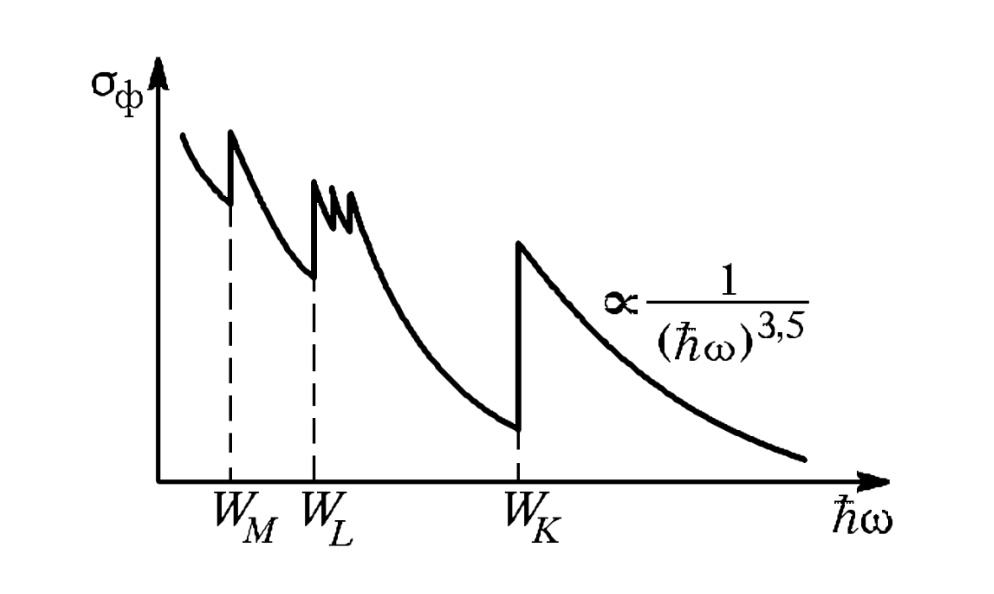
\includegraphics[width = 0.5\textwidth]{img/photo_effect.png}
                    \caption{Зависимость сечения фотоэффекта от энергии $\gamma$-квантов}
                    \label{photo_effect}
                \end{center}
            \end{figure}

        \subsection{Эффект Комптона}

            Это упругое рассеяние фотона на свободном электроне, сопровождающееся изменением длины волны фотона (реально этот процесс происходит на слабо связанных с атомом внешних электронах).

            Вероятность данного процесса определяется энергией $\gamma$-квантов. В области высоких энергий, когда $h\omega \gg mc^2$, сечение вычисляется по формуле:

            $$
            \sigma_k = \pi r^2 \frac{mc^2}{h\omega} \left( \ln \frac{2h\omega}{mc^2} + \frac{1}{2} \right),
            $$

            где $r \simeq 2.8 \cdot 10^{-13}$ см — классический радиус электрона.

            Сечение $\sigma_k$ рассчитано на один свободный электрон и с увеличением энергии фотонов убывает значительно медленнее, чем сечение фотоэффекта.

            Комптоновский коэффициент ослабления $\mu_k$ связан с $\sigma_k$ так же, как $\mu_f$ в случае фотоэффекта. В отличие от фотоэффекта, комптоновское рассеяние не приводит к поглощению $\gamma$-кванта, а только уменьшает его энергию.

        \subsection{Процесс образования электрон-позитронных пар}

            При достаточно высокой энергии гамма-кванта наряду с фотоэффектом и эффектом Комптона может происходить третий вид взаимодействия гамма-квантов с веществом -- образование электрон-позитронных пар.

            Пороговая энергия, необходимая для образования пары:

            $$
                E_{пор} \approx 2mc^2 = 1,022~МэВ
            $$

            Для наблюдения эффекта требуются высокие энергии. Например, $4.7~МэВ$ для $Pb$.


        \subsection{Итого}

    	    В случае опытов, поставленных в хорошей геометрии, при прохождении $\gamma$-лучей через вещество меняет только количество, но не энергия $\gamma$-квантов в пучке, так что коэффициент $\mu$, характеризующий поглощение $\gamma$-квантов в веществе, не зависит от длины пути. Обозначим через $-dN$ число $\gamma$-квантов, выбывших их пучка на пути $dl$. Это число пропорционально имеющемуся их числу $N$ и пройденному пути $dl$. Следовательно,

            \begin{equation}
    	    	\label{eq2}
    	    	-dN = \mu N \, dl.
    	    \end{equation}
    	    Интегрируя уравнение~(\ref{eq2}) от нулевой толщины до заданной, получим
    	    \begin{equation}
    	    	\label{eq3}
    	    	N = N_0 e^{-\mu l}.
    	    \end{equation}

    	    Вообще говоря, в плохой геометрии, когда рассеянные под небольшими углами $\gamma$-кванты остаются в пучке, их спектр с прохождением вещества меняется, поэтому формула~(\ref{eq1}) неприменима. Однако в этом случае она работает лучше, чем можно было ожидать.


    	    Для определения коэффициента ослабления нужно, таким образом, измерить толщину образца $l$, число падающих частиц $N_0$ и число частиц $N$, прошедших через образец за фиксированное время.

    \section{Экспериментальная установка}

    Схема установки, используемой в работе, показана на рис. \ref{setup1}.

    \begin{figure}[h!]
        \begin{center}
            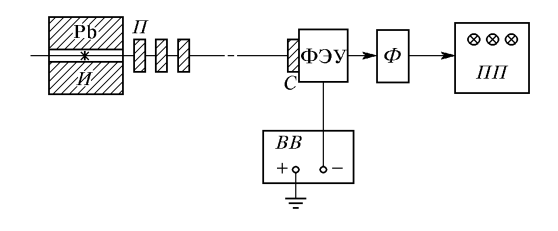
\includegraphics[width = 0.5\textwidth]{img/setup_1.png}
            \caption{Блок-схема установки, используемой для измерения коэффициентов ослабления коэффициентов $\gamma$-лучей: И -- источник $\gamma$-лучей;
                    Pb -- свинцовый контейнер с коллиматорным каналом; П -- набор поглотителей; С -- сцинтиллятор -- кристалл NaI(TI); Ф - формирователь-выпрямитель}
            \label{setup1}
        \end{center}
    \end{figure}

    При недостаточно хорошей геометрии в результаты опытов могут вкрасться существенные погрешности. В установке всегда имеется конечная вероятность того,
    что $\gamma$-квант провзаимодействует в поглотителе несколько раз до того, как попадёт в детектор (рис. \ref{setup2}).
    Чтобы уменьшить число таких случаев, сцинтилляционный счётчик  расположен на большом расстоянии от источника $\gamma$-квантов, а поглотители имеют небольшие размеры.
    Поглотители устанавливаются на некотором расстоянии друг от друга, чтобы испытавшие комптоновское рассеяние и выбывшие из прямого потока кванты с меньшей вероятностью могли в него вернуться.

    \begin{figure}[h!]
        \begin{center}
            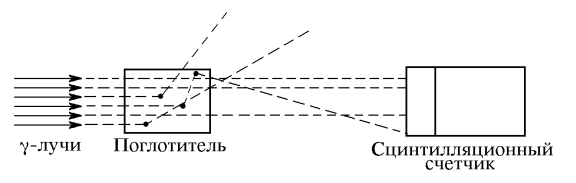
\includegraphics[width = 0.5\textwidth]{img/setup_2.png}
            \caption{Схема рассеяния $\gamma$-квантов в поглотителе}
            \label{setup2}
        \end{center}
    \end{figure}

    \section{Ход работы}

    В начале работы убедились, что установка детектирует $\gamma$-лучи. Для этого провели несколько измерений убирая и возвращая свинцовую пробку.

        \subsection{Измерение интенсивности фона и источника без препятствий}

            \begin{align*}
                I &= \frac{N}{t}; & \sigma_I &= \frac{\sigma_N}{t}
            \end{align*}

            \begin{align*}
                N_{фон} &= 6000 \pm 1000; & t_{фон} &= 180 с; & I_{фон} &= 33 \pm 6 с^{-1} \\
                N_0 &= 120800 \pm 1000; & t_0 &= 10 с; & I_0 &= 12050 \pm 100 с^{-1}
            \end{align*}

        \subsection{Измерение длины образцов}

            Измерили длины образцов при помощи штангенциркуля в том порядке, в котором добавляли при дальнейших измерениях. Рассчитали суммарные длины. Погрешность по формуле $\sigma_{\sum \ell} = \sqrt{\sum{\sigma_{\ell_i}}^2}$. Результаты в таблице \ref{tab:len}.

            \begin{table}[!ht]
                \centering
                \begin{tabular}{|c|c||c|c||c|c|}
                    \hline

                    \multicolumn{2}{|c||}{Pb} & \multicolumn{2}{c||}{Fe} & \multicolumn{2}{c|}{Al}\\ \hline

                    $\ell, мм$ & $\sum \ell, мм$ & $\ell, мм$ & $\sum \ell, мм$ & $\ell, мм$ & $\sum \ell, мм$\\ \hline
                    $4.80 \pm 0.10$ & $4.80 \pm 0.10$ & $10.10 \pm 0.10$ & $10.10 \pm 0.10$ & $20.10 \pm 0.02$ & $20.10 \pm 0.02$\\ \hline
                    $5.00 \pm 0.10$ & $9.8 \pm 0.1$ & $10.10 \pm 0.10$ & $20.2 \pm 0.1$ & $20.22 \pm 0.02$ & $40.32 \pm 0.03$\\ \hline
                    $5.00 \pm 0.10$ & $14.8 \pm 0.2$ & $10.00 \pm 0.10$ & $30.2 \pm 0.2$ & $20.00 \pm 0.02$ & $60.32 \pm 0.03$\\ \hline
                    $5.00 \pm 0.10$ & $19.8 \pm 0.2$ & $10.00 \pm 0.10$ & $40.2 \pm 0.2$ & $20.12 \pm 0.02$ & $80.44 \pm 0.04$\\ \hline
                    $4.50 \pm 0.10$ & $24.3 \pm 0.2$ & $9.90 \pm 0.10$ & $50.1 \pm 0.2$ & $20.30 \pm 0.02$ & $100.74 \pm 0.04$\\ \hline
                    $4.90 \pm 0.10$ & $29.2 \pm 0.2$ & $10.00 \pm 0.10$ & $60.1 \pm 0.2$ & $20.00 \pm 0.02$ & $120.74 \pm 0.05$\\ \hline
                    $4.60 \pm 0.10$ & $33.8 \pm 0.3$ & $10.30 \pm 0.10$ & $70.4 \pm 0.3$ & $20.00 \pm 0.02$ & $140.74 \pm 0.05$\\ \hline
                    $4.70 \pm 0.10$ & $38.5 \pm 0.3$ & $10.30 \pm 0.10$ & $80.7 \pm 0.3$ & $20.20 \pm 0.02$ & $160.94 \pm 0.06$\\ \hline
                    $5.20 \pm 0.10$ & $43.7 \pm 0.3$ & $10.10 \pm 0.10$ & $90.8 \pm 0.3$ & $20.00 \pm 0.02$ & $180.94 \pm 0.06$\\ \hline

                \end{tabular}
                \caption{Результаты измерений длин образцов и суммарных длин препятствий}
                \label{tab:len}
            \end{table}

        \subsection{Исследования поглощения $\gamma$-лучей}

            Измерили число частиц, попадающих в счётчик за некоторое время, в зависимости от суммарной толщины препятствий. Исследовались 3 материала: свинец, железо и алюминий. Результаты в таблице \ref{tab:N}.

            \begin{table}[!ht]
                \centering
                \begin{tabular}{|c|c|c||c|c|c||c|c|c|}
                    \hline

                    \multicolumn{3}{|c||}{Pb} & \multicolumn{3}{c||}{Fe} & \multicolumn{3}{c|}{Al}\\ \hline
                    $N*10^3$ & $t, с$ & $\sum \ell, мм$ & $N*10^3$ & $t, с$ & $\sum \ell, мм$ & $N*10^3$ & $t, с$ & $\sum \ell, мм$\\ \hline
                    $130.8 \pm 1.0$ & $20$ & $4.80 \pm 0.10$ & $135.8 \pm 1.0$ & $20$ & $10.10 \pm 0.10$ & $157.3 \pm 1.0$ & $20$ & $20.10 \pm 0.02$\\ \hline
                    $124.0 \pm 1.0$ & $30$ & $9.8 \pm 0.1$ & $126.1 \pm 1.0$ & $30$ & $20.2 \pm 0.1$ & $221.7 \pm 1.0$ & $40$ & $40.32 \pm 0.03$\\ \hline
                    $140.7 \pm 1.0$ & $60$ & $14.8 \pm 0.2$ & $108.0 \pm 1.0$ & $45$ & $30.2 \pm 0.2$ & $147.6 \pm 1.0$ & $40$ & $60.32 \pm 0.03$\\ \hline
                    $126.9 \pm 1.0$ & $90$ & $19.8 \pm 0.2$ & $112.1 \pm 1.0$ & $80$ & $40.2 \pm 0.2$ & $99.7 \pm 1.0$ & $40$ & $80.44 \pm 0.04$\\ \hline
                    $102.2 \pm 1.0$ & $120$ & $24.3 \pm 0.2$ & $103.6 \pm 1.0$ & $120$ & $50.1 \pm 0.2$ & $102.9 \pm 1.0$ & $60$ & $100.74 \pm 0.04$\\ \hline
                    $96.6 \pm 1.0$ & $180$ & $29.2 \pm 0.2$ & $93.6 \pm 1.0$ & $180$ & $60.1 \pm 0.2$ & $106.1 \pm 1.0$ & $90$ & $120.74 \pm 0.05$\\ \hline
                    $66.3 \pm 1.0$ & $180$ & $33.8 \pm 0.3$ & $59.5 \pm 1.0$ & $180$ & $70.4 \pm 0.3$ & $99.3 \pm 1.0$ & $120$ & $140.74 \pm 0.05$\\ \hline
                    $42.7 \pm 1.0$ & $180$ & $38.5 \pm 0.3$ & $38.8 \pm 1.0$ & $180$ & $80.7 \pm 0.3$ & $105.8 \pm 1.0$ & $180$ & $160.94 \pm 0.06$\\ \hline
                    $27.8 \pm 1.0$ & $180$ & $43.7 \pm 0.3$ & $26.6 \pm 1.0$ & $180$ & $90.8 \pm 0.3$ & $75.8 \pm 1.0$ & $180$ & $180.94 \pm 0.06$\\ \hline

                \end{tabular}
                \caption{Результаты измерений числа частиц, попавших в счётчик, в зависимости от суммарной длины препятствий}
                \label{tab:N}
            \end{table}

            Из уравнения (\ref{eq3}) ожидается экспоненциальный характер поглощения. Построим графики и определим линейные коэффициенты поглощения $\mu$.

            По оси абсцисс отложим суммарную длину препятствия, по оси ординат $ln\frac{I_0 - I_{фон}}{I - I_{фон}}$. Коэффициент наклона прямой и будет равен $\mu$.

            Результаты представлены в таблице \ref{tab:mu}.

            \begin{figure}[ht!]
                \begin{center}
                    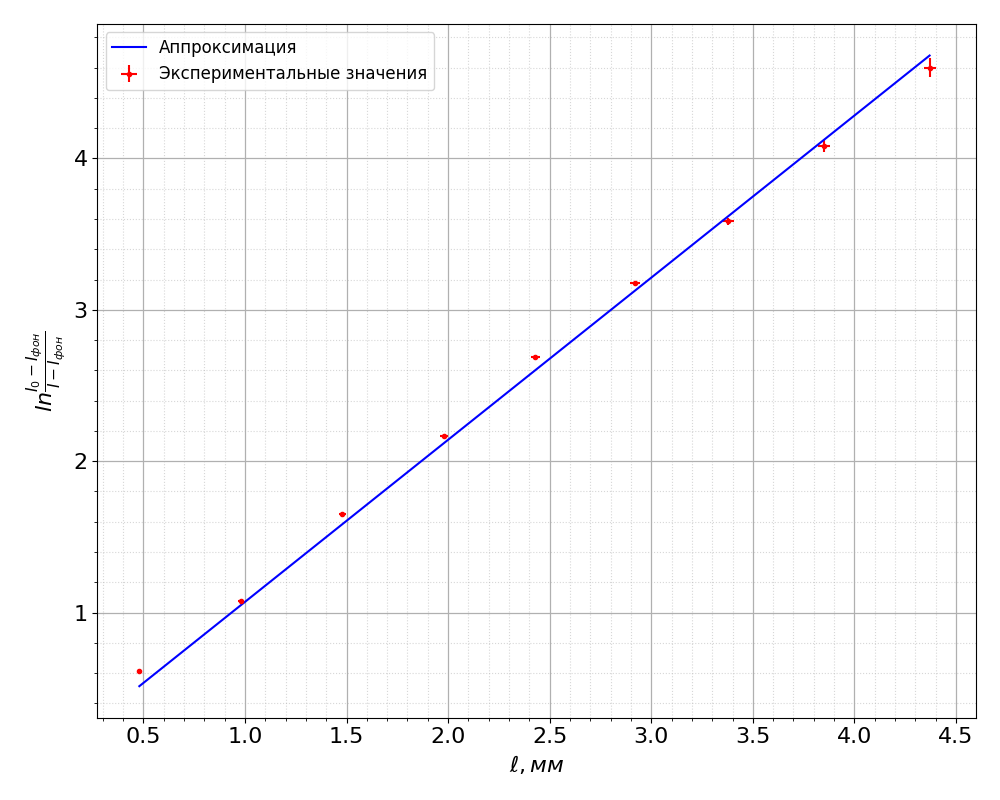
\includegraphics[width = 0.7\textwidth]{img/Pb.png}
                    \caption{Зависимость интенсивности прошедшего излучения от длины препятствий для свинца}
                    \label{plot:Pb}
                \end{center}
            \end{figure}

            \begin{figure}[ht!]
                \begin{center}
                    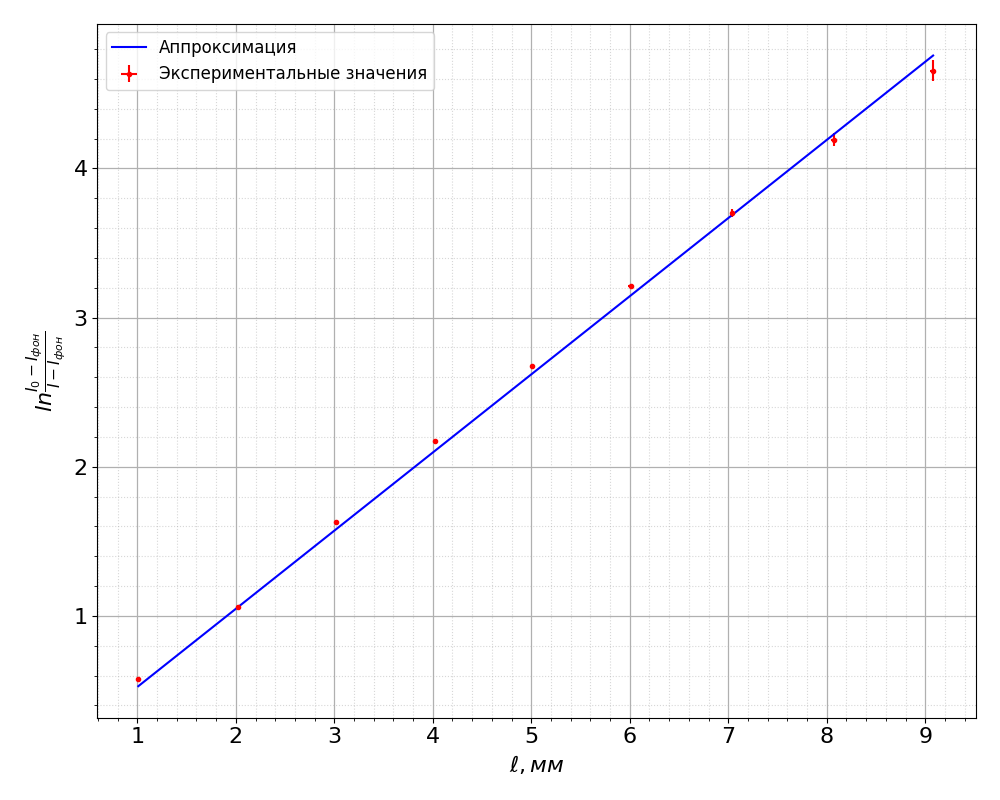
\includegraphics[width = 0.7\textwidth]{img/Fe.png}
                    \caption{Зависимость интенсивности прошедшего излучения от длины препятствий для железа}
                    \label{plot:Fe}
                \end{center}
            \end{figure}

            \begin{figure}[ht!]
                \begin{center}
                    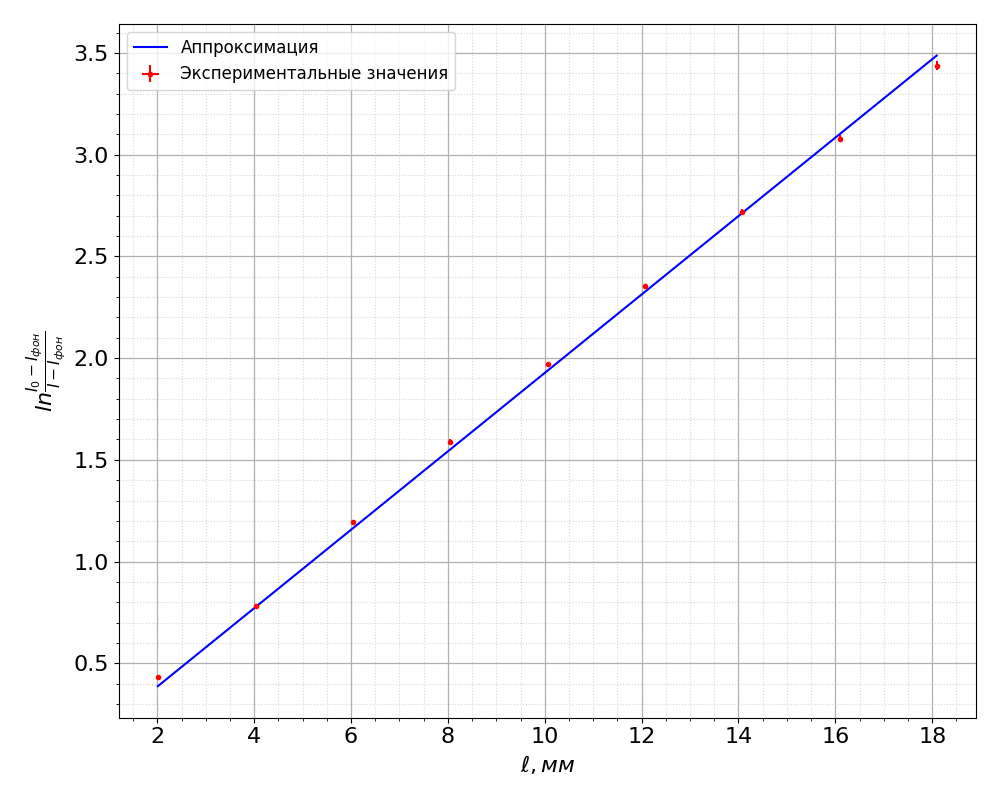
\includegraphics[width = 0.8\textwidth]{img/Al.png}
                    \caption{Зависимость интенсивности прошедшего излучения от длины препятствий для алюминия}
                    \label{plot:Al}
                \end{center}
            \end{figure}

            \begin{table}[!ht]
                \centering
                \begin{tabular}{|c|c|c|c|c|}
                    \hline

                     & Pb & Fe & Al\\ \hline
                    $\mu,~см^{-1}$ & $1.071 \pm 0.008$ & $0.524 \pm 0.003$ & $0.193 \pm 0.001$\\ \hline

                \end{tabular}
                \caption{Линейные коэффициенты поглощения $\mu$}
                \label{tab:mu}
            \end{table}


            Определим $\mu'$, который зависит от массы пройденного вещества на единицу площади, из следующих соображений:
            \begin{align*}
                \mu' m_1 = \mu \ell \Rightarrow \mu' = \mu \frac{\ell}{m_1} &= \frac{\mu}{\rho}, & \sigma_{\mu'} &= \frac{\sigma_{\mu}}{\rho}
            \end{align*}

            Результаты в таблице \ref{tab:mu_m1}.

            \begin{table}[!ht]
                \centering
                \begin{tabular}{|c|c|c|c|}
                    \hline
                     & Pb & Fe & Al\\ \hline
                    $\rho,~г/см^3$ & $11.35$ & $7.87$ & $2.7$\\ \hline
                    $\mu'*10^{-3},~см^2/г$ & $94.3 \pm 0.7$ & $66.6 \pm 0.4$ & $71.4 \pm 0.4$\\ \hline
                 \end{tabular}
                \caption{Линейные коэффициенты поглощения $\mu'$}
                \label{tab:mu_m1}
            \end{table}

        \subsection{Определение энергии фотона по коэффициенту поглощения}

            По данной таблице \ref{tab:lab_E} определим среднюю энергию фотона. Для этого аппроксимируем зависимость $\frac{1}{E}(\mu)$ кривой $y = ax^2 + bx + c$. Итоговые коэффициенты в таблице \ref{tab:approx_coeffs}, график на рис. \ref{plot:tab_approx}.

            По полученным кривым получим значения энергий фотонов (таблица \ref{tab:E}). Погрешность по формуле:
            \begin{align*}
                E &= \frac{1}{a\mu^2 + b\mu + c} & \sigma_E &= \frac{\sqrt{\left( 2ax + b \right)^2 \sigma_{\mu}^2 + \left( \mu^2 \right)^2 \sigma_a^2 + \left( \mu \right)^2 \sigma_b^2 + \sigma_c^2}}{\left( a\mu^2 + b\mu + c \right)^2}
            \end{align*}

            \begin{table}[!ht]
                \centering
                \begin{tabular}{|c|c|c|c|}
                    \hline

                    \multirow{2}{*}{$E_{фотон}, МэВ$} & \multicolumn{3}{c|}{$\mu, см^{-1}$} \\ \cline{2-4}
                     & Pb & Fe & Al\\ \hline
                    $0.4$ & $2.63$ & $0.74$ & $0.25$\\ \hline
                    $0.5$ & $1.83$ & $0.662$ & $0.228$\\ \hline
                    $0.6$ & $1.42$ & $0.606$ & $0.21$\\ \hline
                    $0.7$ & $1.17$ & $0.563$ & $0.196$\\ \hline
                    $0.8$ & $1.01$ & $0.528$ & $0.184$\\ \hline
                    $0.9$ & $0.891$ & $0.498$ & $0.175$\\ \hline
                    $1.0$ & $0.806$ & $0.472$ & $0.166$\\ \hline
                    $1.1$ & $0.74$ & $0.45$ & $0.158$\\ \hline

                \end{tabular}
                \caption{Табличные значения энергий фотонов и коэффициентов поглощений для трёх материалов}
                \label{tab:lab_E}
            \end{table}

            \begin{figure}[ht!]
                \begin{center}
                    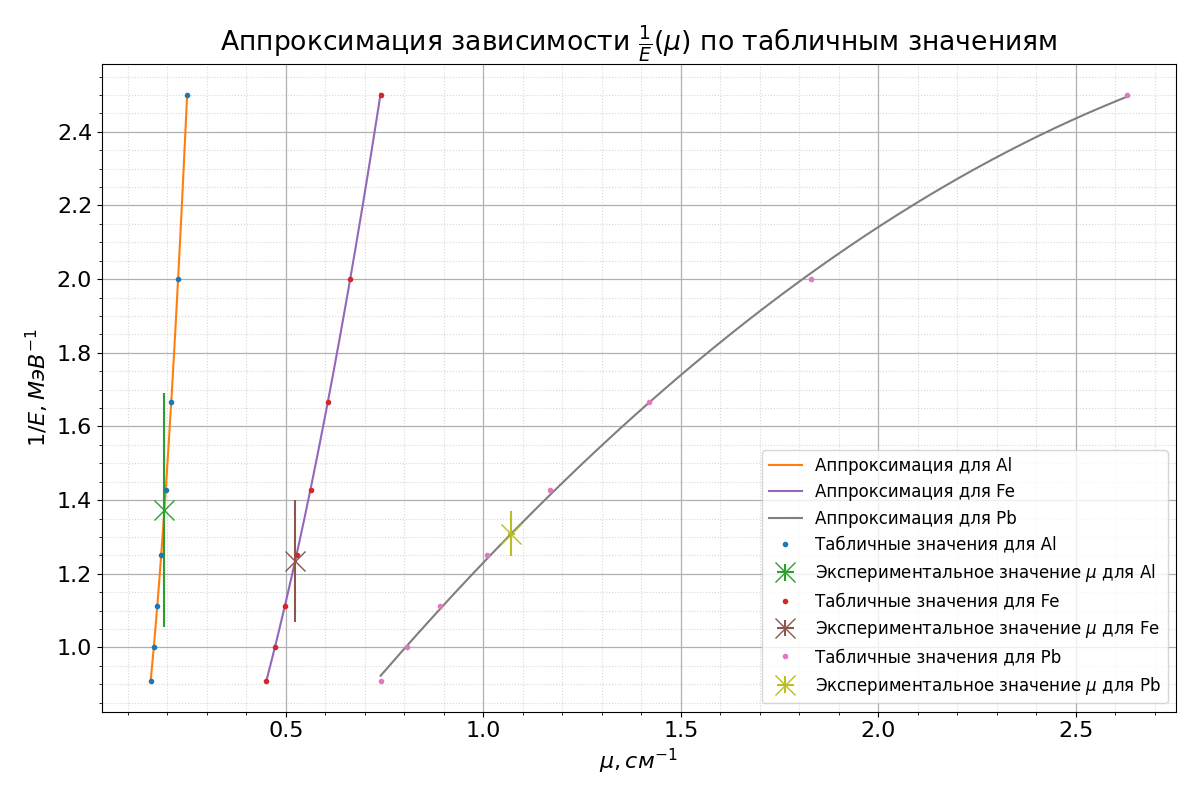
\includegraphics[width = 0.8\textwidth]{img/attenuation_factor_plot.png}
                    \caption{Аппроксимация табличных значений}
                    \label{plot:tab_approx}
                \end{center}
            \end{figure}

            \begin{table}[!ht]
                \centering
                \begin{tabular}{|c|c|c|c|}
                    \hline

                     & Pb & Fe & Al\\ \hline
                    $a$ & $68 \pm 3$ & $4.8 \pm 0.2$ & $-0.21 \pm 0.01$\\ \hline
                    $b$ & $-10 \pm 1$ & $-0.3 \pm 0.3$ & $1.55 \pm 0.05$\\ \hline
                    $c$& $0.9 \pm 0.1$ & $0.04 \pm 0.07$ & $-0.11 \pm 0.03$\\ \hline

                \end{tabular}
                \caption{Коэффициенты аппроксимации}
                \label{tab:approx_coeffs}
            \end{table}

            \begin{table}[!ht]
                \centering
                \begin{tabular}{|c|c|c|c|c|}
                    \hline

                     & Pb & Fe & Al & Среднее\\ \hline
                    $E,~МэВ$ & $0.7 \pm 0.2$ & $0.81 \pm 0.11$ & $0.76 \pm 0.04$ & $0.77 \pm 0.11$\\ \hline

                \end{tabular}
                \caption{Средняя энергия $\gamma$-лучей по коэффициентам поглощения}
                \label{tab:E}
            \end{table}

    \section{Вывод}

        В работе изучено поглощение $\gamma$-лучей в свинце, железе и алюминии. Экспериментально получены коэффициенты поглощения материалов. По коэффициентам получена средняя энергия $\gamma$-лучей источника.

        \begin{table}[!ht]
            \centering
            \begin{tabular}{|c|c|c|c|c|}
                \hline

                 & Pb & Fe & Al & \multirow{3}{*}{Среднее}\\ \cline{1-4}
                $\mu,~см^{-1}$ & $1.071 \pm 0.008$ & $0.524 \pm 0.003$ & $0.193 \pm 0.001$ &\\ \cline{1-4}
                $\mu'*10^{-3},~см^2/г$ & $94.3 \pm 0.7$ & $66.6 \pm 0.4$ & $66.6 \pm 0.4$ &\\ \hline
                $E,~МэВ$ & $0.7 \pm 0.2$ & $0.81 \pm 0.11$ & $0.76 \pm 0.04$ & $0.77 \pm 0.11$\\ \hline

            \end{tabular}
            \caption{Результаты работы}
            \label{tab:res}
        \end{table}

        Источником служил $^{137}Cs$, энергия $\gamma$-кванта для которого равна $0.662~МэВ$. Рассчитанное значение в пределах погрешности совпадает.

\end{document}

